% ----------------------------------------------------------
% Testes
% 
% ----------------------------------------------------------

\chapter[Testes]{Testes}

Nesse capitulo, serão descritos os planejamentos de testes com a descrição de todos os casos de testes envolvidos na aplicação.

\section{Planos de Testes}

Para uma melhor eficácia dos testes, é de suma importância o planejamento dos testes, no desenvolvimento de software é imprescindível para o projeto ser bem sucedido. De acordo com o grande crescimento e avanço tecnológico se torna cada vez mais necessário entregar softwares seguros, de altíssima qualidade e confiáveis torna-se uma prioridade absoluta. 
Após todas as telas serem finalizadas, começamos a planejar os testes necessários para entregar um software com um ótimo funcionamento, o primeiro teste realizado foi no sistema de login, no qual, testamos a criação da conta, a redefinição da senha e o login no aplicativo. No segundo teste, verificamos o menu principal, no qual foram analisados os controles de receita, os controles de despesas e a importação da fatura em PDF. 


\section{Cenários de Testes}

\subsection{Sistema de Login}

Testes realizados para testar e validar o funcionamento do sistema de login e dos subprogramas.

\vspace{\baselineskip}
\vspace{\baselineskip}
\vspace{\baselineskip}
\vspace{\baselineskip}
\vspace{\baselineskip}
\vspace{\baselineskip}
\vspace{\baselineskip}
\vspace{\baselineskip}
\vspace{\baselineskip}
\vspace{\baselineskip}
\vspace{\baselineskip}

\subsubsection{Caso de Teste 0001 - Realizar Login}

Teste realizado para a validação de usuário e senha a partir do menu principal, conforme figura 35.

    \begin{center}
        \begin{minipage}{\textwidth}
            \centering
            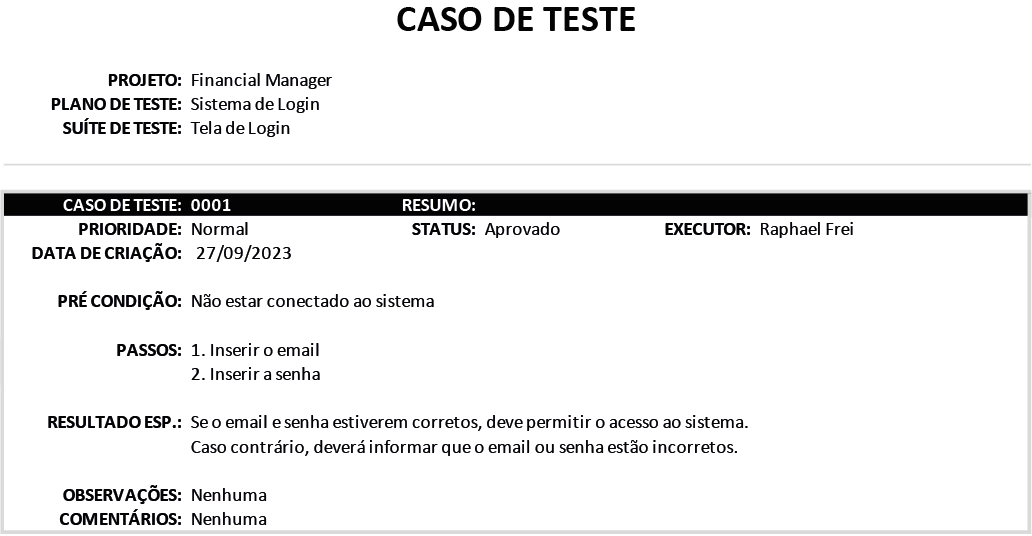
\includegraphics[scale=0.8]{figs/caso-testes-0001.png}
            \captionof{figure}{Caso de Teste da Tela de Login}
            \label{fig:figura35}
        \end{minipage}
    \end{center} 

\subsubsection{Caso de Teste 0002 - Recuperar a Senha}

Teste realizado para a recuperação de senha do usuário, conforme figura 36.

    \begin{center}
        \begin{minipage}{\textwidth}
            \centering
            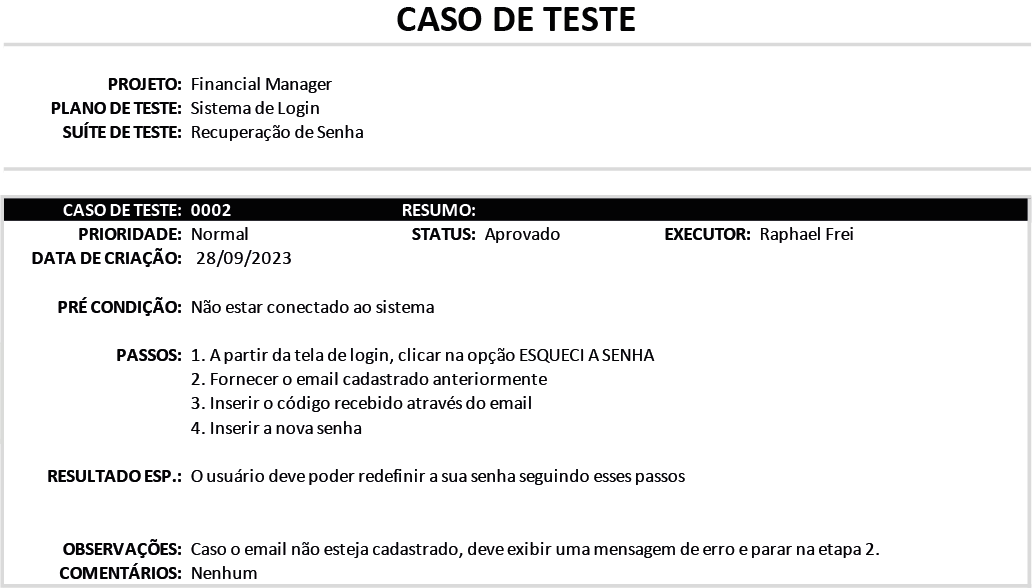
\includegraphics[scale=0.8]{figs/caso-testes-0002.png}
            \captionof{figure}{Caso de Teste da Recuperação de Senha}
            \label{fig:figura36}
        \end{minipage}
    \end{center} 

\subsubsection{Caso de Teste 0003 - Cadastro de Conta}

Teste realizado para o cadastro de novas contas, descrito na figura 37.

    \begin{center}
        \begin{minipage}{\textwidth}
            \centering
            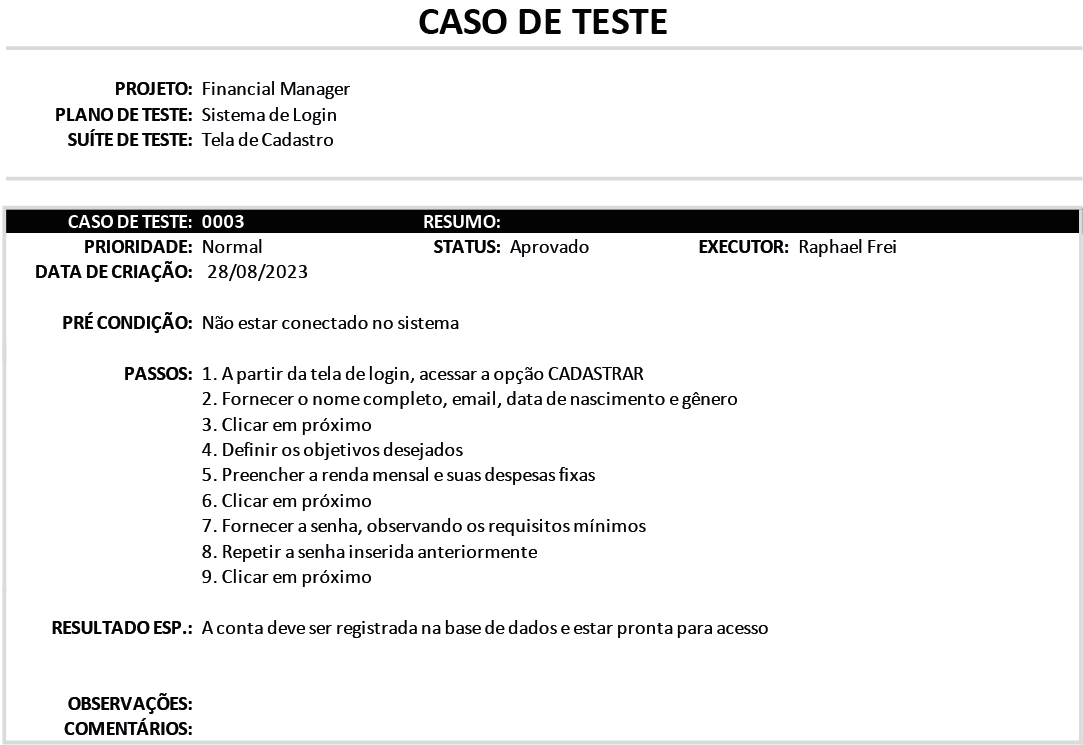
\includegraphics[scale=0.8]{figs/caso-testes-0003.png}
            \captionof{figure}{Caso de Teste da Tela de Cadastro}
            \label{fig:figura37}
        \end{minipage}
    \end{center} 

\subsubsection{Caso de Teste 0004 - Recuperar Conta}

Teste realizado para o processo de recuperação do acesso, descrito na figura 38.

    \begin{center}
        \begin{minipage}{\textwidth}
            \centering
            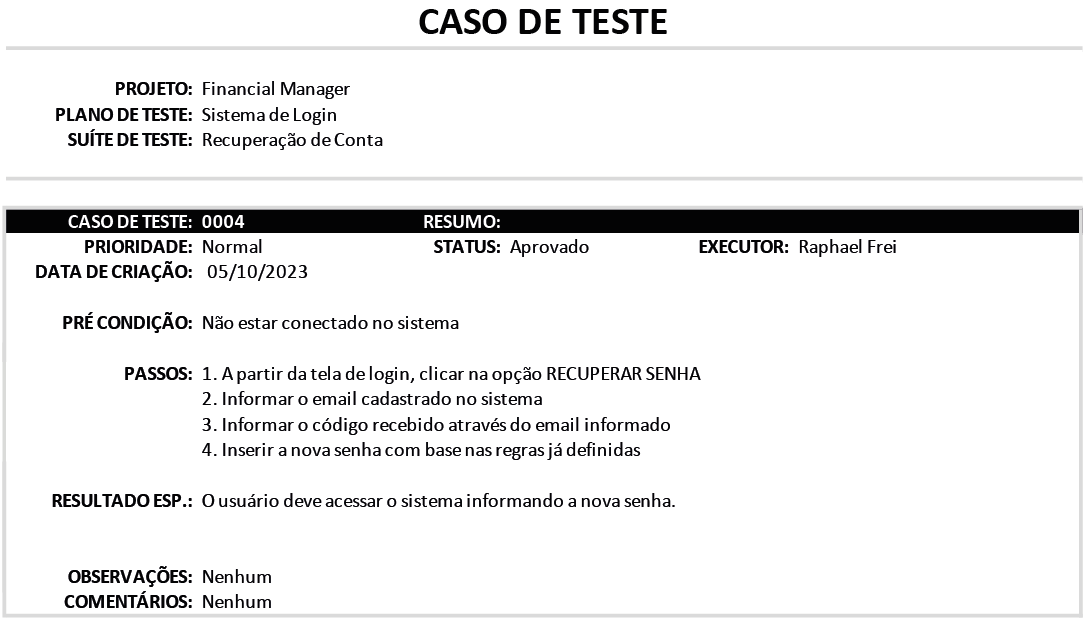
\includegraphics[scale=0.75]{figs/caso-testes-0004.png}
            \captionof{figure}{Caso de Teste da Recuperação de Conta}
            \label{fig:figura38}
        \end{minipage}
    \end{center} 
    
\subsection{Menu Principal}

Teste realizado para testar e validar o funcionamento do menu principal e dos subprogramas.

\subsubsection{Caso de Teste 0005 - Adicionar Receita}

Teste realizado para a tela de adição de receitas, descrito na figura 39.

    \begin{center}
        \begin{minipage}{\textwidth}
            \centering
            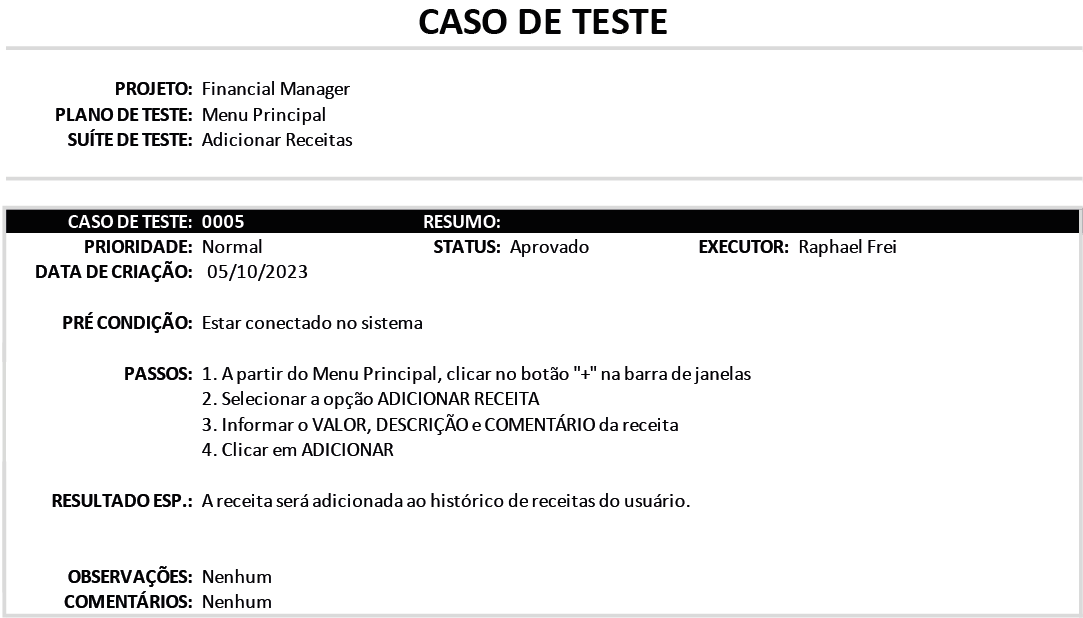
\includegraphics[scale=0.8]{figs/caso-testes-0005.png}
            \captionof{figure}{Caso de Teste para Adicionar Receita}
            \label{fig:figura39}
        \end{minipage}
    \end{center} 

\subsubsection{Caso de Teste 0006 - Editar Receita}

Teste realizado para a tela de edição de receitas, conforme figura 40.

    \begin{center}
        \begin{minipage}{\textwidth}
            \centering
            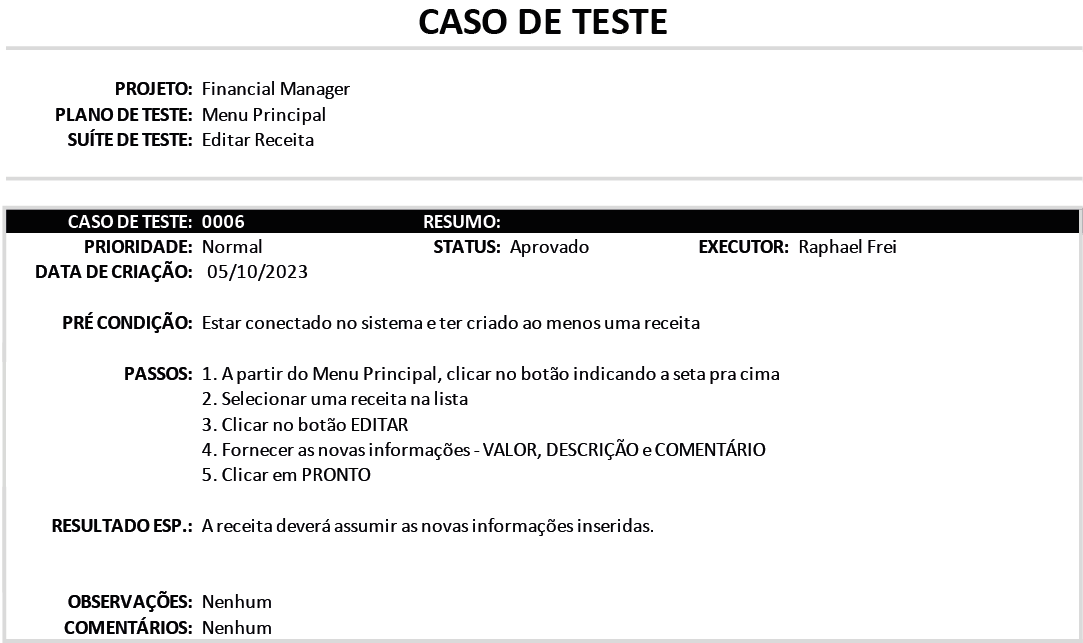
\includegraphics[scale=0.5]{figs/caso-testes-0006.png}
            \captionof{figure}{Caso de Teste para Editar Receita}
            \label{fig:figura40}
        \end{minipage}
    \end{center} 

\subsubsection{Caso de Teste 0007 - Excluir Receita}

Teste realizado para a tela de exclusão de receitas, conforme figura 41.

    \begin{center}
        \begin{minipage}{\textwidth}
            \centering
            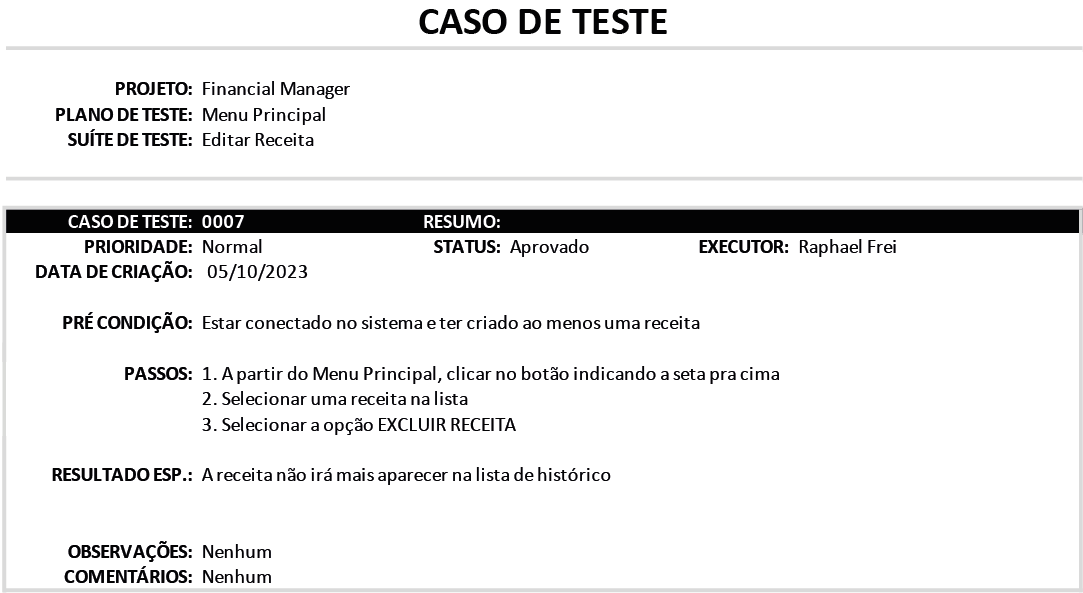
\includegraphics[scale=0.8]{figs/caso-testes-0007.png}
            \captionof{figure}{Caso de Teste para Excluir Receita}
            \label{fig:figura41}
        \end{minipage}
    \end{center} 

\subsubsection{Caso de Teste 0008 - Importar PDF}

Teste realizado para o sistema de importação de fatura em PDF, conforme figura 42.

    \begin{center}
        \begin{minipage}{\textwidth}
            \centering
            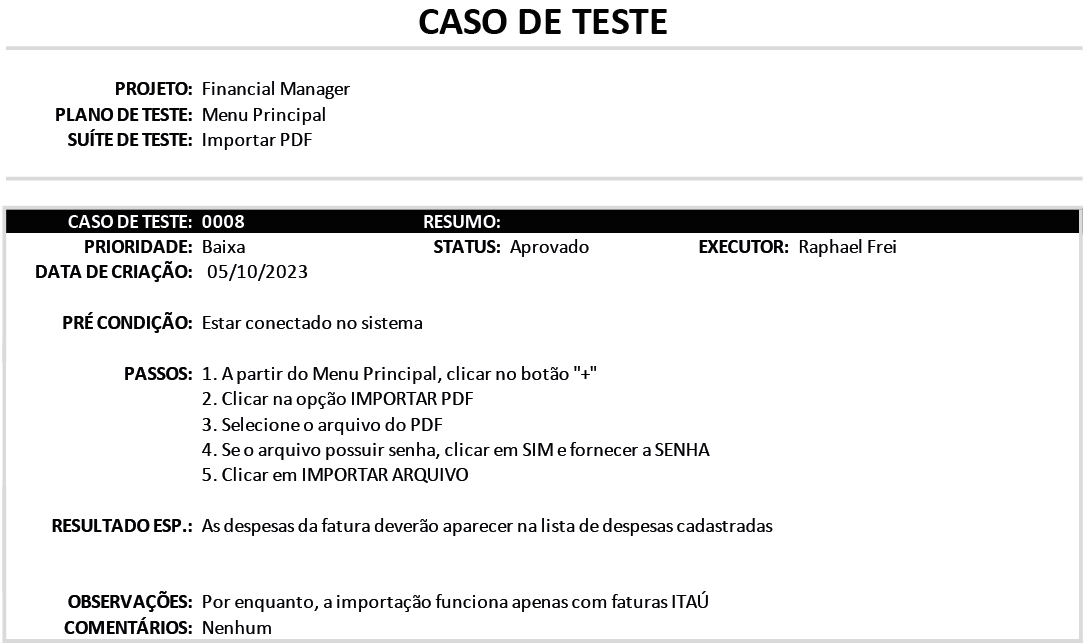
\includegraphics[scale=0.8]{figs/caso-testes-0008.png}
            \captionof{figure}{Caso de Teste para Importar PDF}
            \label{fig:figura42}
        \end{minipage}
    \end{center} 

\subsubsection{Caso de Teste 0009 - Adicionar Despesa}

Teste realizado para a tela de adição de despesas, conforme figura 43.

    \begin{center}
        \begin{minipage}{\textwidth}
            \centering
            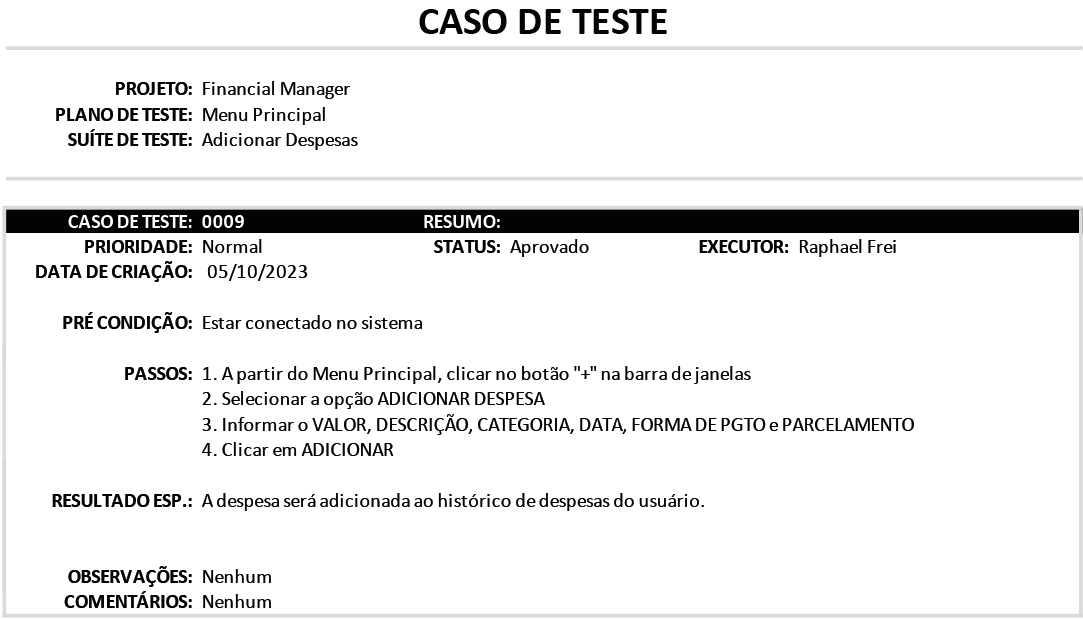
\includegraphics[scale=0.8]{figs/caso-testes-0009.png}
            \captionof{figure}{Caso de Teste para Adicionar Despesa}
            \label{fig:figura43}
        \end{minipage}
    \end{center} 

\subsubsection{Caso de Teste 0010 - Editar Despesa}

Teste realizado para a tela de edição de despesas, conforme figura 44.

    \begin{center}
        \begin{minipage}{\textwidth}
            \centering
            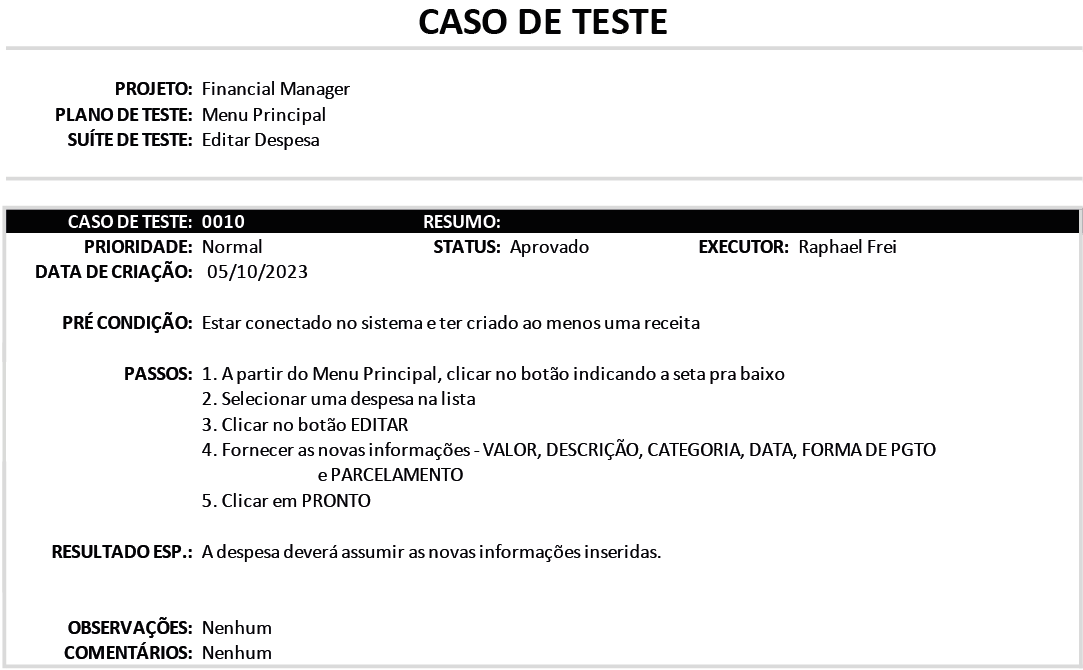
\includegraphics[scale=0.8]{figs/caso-testes-0010.png}
            \captionof{figure}{Caso de Teste para Editar Despesa}
            \label{fig:figura44}
        \end{minipage}
    \end{center} 

\subsubsection{Caso de Teste 0011 - Excluir Despesa}

Teste realizado para a tela de exclusão de despesas, conforme figura 45.

    \begin{center}
        \begin{minipage}{\textwidth}
            \centering
            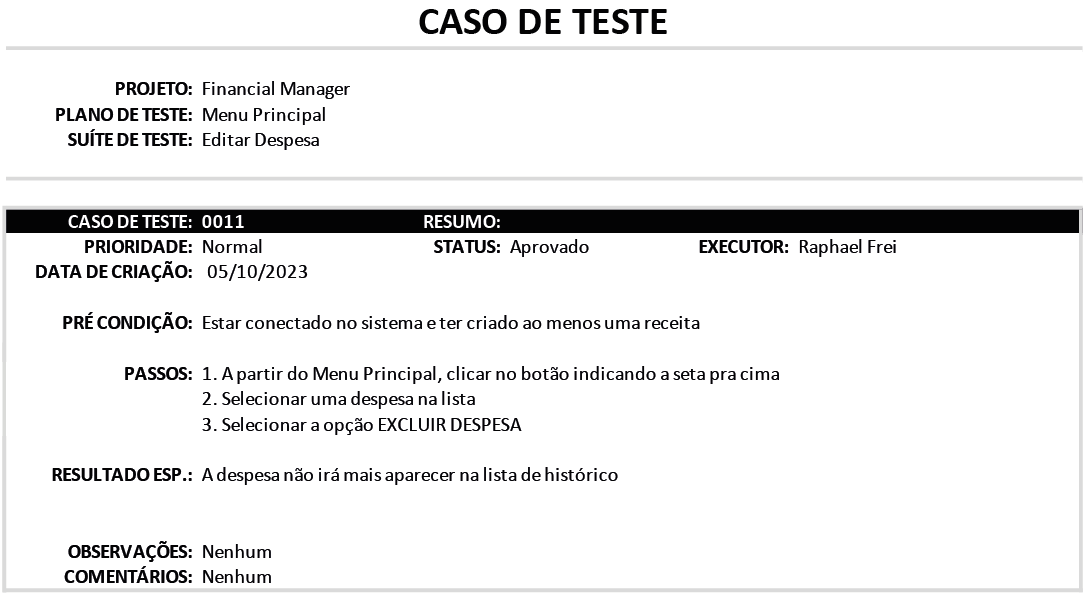
\includegraphics[scale=0.8]{figs/caso-testes-0011.png}
            \captionof{figure}{Caso de Teste para Excluir Despesa}
            \label{fig:figura45}
        \end{minipage}
    \end{center} 
